\chapter{Analyse aktueller Lösungen}
\label{ch:analysis}
Bevor mit dem Entwurf des Konzepts und der Implementierung der Anwendung begonnen werden kann, muss die Ist-Situation analysiert werden.
Die Erkenntnisse, die bei der Analyse der aktuellen Lösungen und deren Probleme gewonnen werden, können im Anschluss in die Konzeption und die Implementierung einfließen.

\section{Aufstellen der Anforderungen}
In diesem Abschnitt werden die Anforderungen an ein System zur Erstellung von Indoor Maps beschrieben.
Dabei wird besonders die Situation des genannten Anwendungsfalls aus dem \autoref{sec:problems} der Einleitung berücksichtigt.
Es handelt sich um einen Vermieter einer kleinen Einkaufspassage, welcher Indoor Maps und eine Innenraumnavigation für die Besucher der Einkaufspassage anbieten möchte.
Für einen solchen Fall sind die folgenden Anforderungen ausschlaggebend.
\begin{description}
	\item[Preisliche Stemmbarkeit]
	Für den Vermieter sollte eine in Frage kommende Lösung preislich stemmbar sein.
	Bei der Bereitstellung von Indoor Maps handelt es sich nicht um eine kritische Dienstleistung für die Besucher, sondern um ein mögliches Angebot.
	Sind die Kosten für die Lösung zu hoch, so ist das Verhältnis zwischen dem Preis und der erhaltenden Leistungen nicht ausgewogen und der Vermieter zieht die Lösung nicht in Erwägung.\pbreak%
	%
	Eine mit Kosten verbundene Lösung der Situation des Vermieters entsprechend ist für den Vermieter daher von hoher Relevanz.
	\item[Schnelle Einarbeitungszeit]
	Bei der Bereitstellung von Indoor Maps handelt es sich für den Vermieter um ein einmaliges Projekt.
	Es würde nicht im Interesse des Vermieters stehen, wenn er sich zu Beginn in die Anwendung einarbeiten muss.
	Die Zeit für die Einarbeitung ist wieder mit Kosten verbunden, da Arbeitszeit in Anspruch genommen wird und dadurch die Frage des ersten Punktes der preislichen Stemmbarkeit wieder eintritt.\pbreak%
	%
	Eine Einarbeitungszeit sollte sehr kurz bis gar nicht vorhanden sein, sodass der Vermieter sofort mit dem Erstellen der Kartendaten beginnen kann.
	\item[Leichte und nachvollziehbare Bedienung]
	In direkter Beziehung zur schnellen Einarbeitungszeit sollte auch die leichte und nachvollziehbare Bedienung stehen.
	Im Idealfall funktioniert die Erstellung der Kartendaten nach dem ``What You See Is What You Get``-Prinzip (WYSIWYG), zu Deutsch: Was du siehst ist was du bekommst.
	Dadurch ist es dem Anwender nachvollziehbar was das Ergebnis ist, da die Darstellung während der Bearbeitung dem fertigen Produkt entspricht.
	Sind die Aktionen während der Bearbeitung der Kartendaten nicht nachvollziehbar, kann es dazu führen, dass der Vermieter den Überblick über das Projekt verliert.\pbreak%
	%
	Der Vermieter sollte zu keinem Zeitpunkt über das Ausführen einer Aktion nachdenken müssen.
	Es sollte zu jeder Zeit klar sein, welche Funktion hinter welchem Button liegt und was sich im Projekt verändert, wenn diese Funktion genutzt wird.
	\item[Mobile Nutzung]
	Die Nutzung der Anwendung sollte für den Vermieter mobil möglich sein.
	Während Vermessungsbüros die Räumlichkeiten komplett ausmessen und die Kartendaten im Anschluss an einem festen Standort erstellen, hat der Vermieter nicht die Möglichkeit die Räumlichkeiten komplett auszumessen.
	Ein immer wiederkehrender Weg zwischen Räumlichkeiten und der Stelle, an der die Kartendaten eingetragen werden, wäre anstrengend und unattraktiv für den Vermieter.\pbreak%
	%
	Es sollte für den Vermieter möglich sein, die Räumlichkeiten zu vermessen und die Kartendaten auch direkt dort einzutragen.
	Die Mobilität erlaubt es dem Vermieter, schnell die Orte zu wechseln und trotzdem weiterzuarbeiten.\pagebreak
\end{description}
Die aufgestellten Anforderungen werden mit den sich aktuell auf dem Markt befindlichen Lösungen verglichen.
So können Übereinstimmungen und Probleme erkannt werden und im Anschluss in die Konzeption einfließen.

\section{Softwarelösungen}
Bei den möglichen Lösungen wird zwischen \emph{Softwarelösungen} und \emph{Dienstleistungslösungen} unterschieden.
Ersteres beschreibt jegliche Software, mit welcher die benötigten Kartendaten erzeugt werden können und zweiteres Lösungen, die keine eigene Arbeit beanspruchen.
In diesem Abschnitt werden einige Softwarelösungen vorgestellt und analysiert.

\subsection{QGIS}
Bei dem Softwareprojekt QGIS handelt es sich um ein professionelles Geographisches-Informationssystem, welches bis zum Release der Version 2.0 noch \emph{Quantum GIS} hieß \parencite{QGI2013, SUT2013}.
\begin{figure}[h!]
	\centering
	\vspace{15pt}
	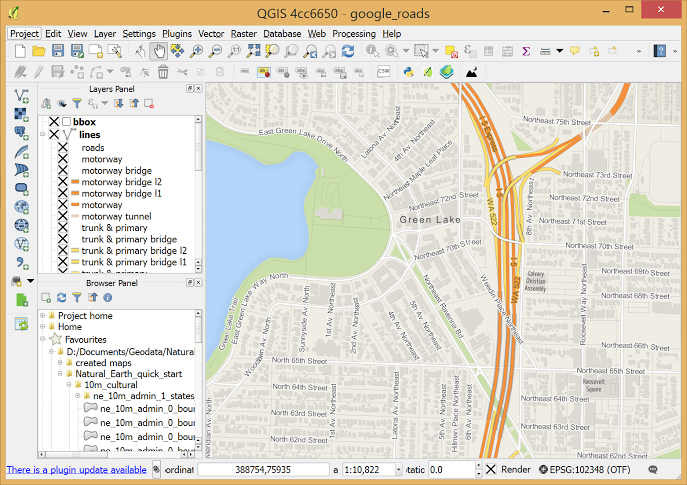
\includegraphics[scale=0.5]{images/analysis/qgis.png}
	\caption{Bearbeitungsansicht in QGIS \parencite{QGI}}
	\label{fig:analysis-qgis}
\end{figure}
\analysisresults{
Da QGIS ein Open-Source Projekt ist, kann man die Anwendung kostenlos auf der eigenen Website herunterladen \parencite{QGI2020}.
Die Anwendung steht für alle gängigen Betriebssystem zur Verfügung und obwohl QGIS kostenlos ist, nimmt die \emph{QGIS Anwendergruppe Deutschland} spenden an \parencite{QGI2020a}.
}{
Bei dieser Software handelt es sich um eine professionelle Anwendung zur Bearbeitung von Kartendaten jeglicher Art.
Diese Komplexität trägt dazu bei, dass die Einarbeitung in die Software Zeit in Anspruch nimmt.
QGIS bietet eine ausführliche und somit auch lange Dokumentation zur Anwendung an \parencite{QGI2020b}.
}{
Nach der Installation und dem Öffnen ist nicht klar, wie man ein neuen Projekt erstellen beziehungsweise bearbeiten kann.
\begin{figure}[h!]
	\centering
	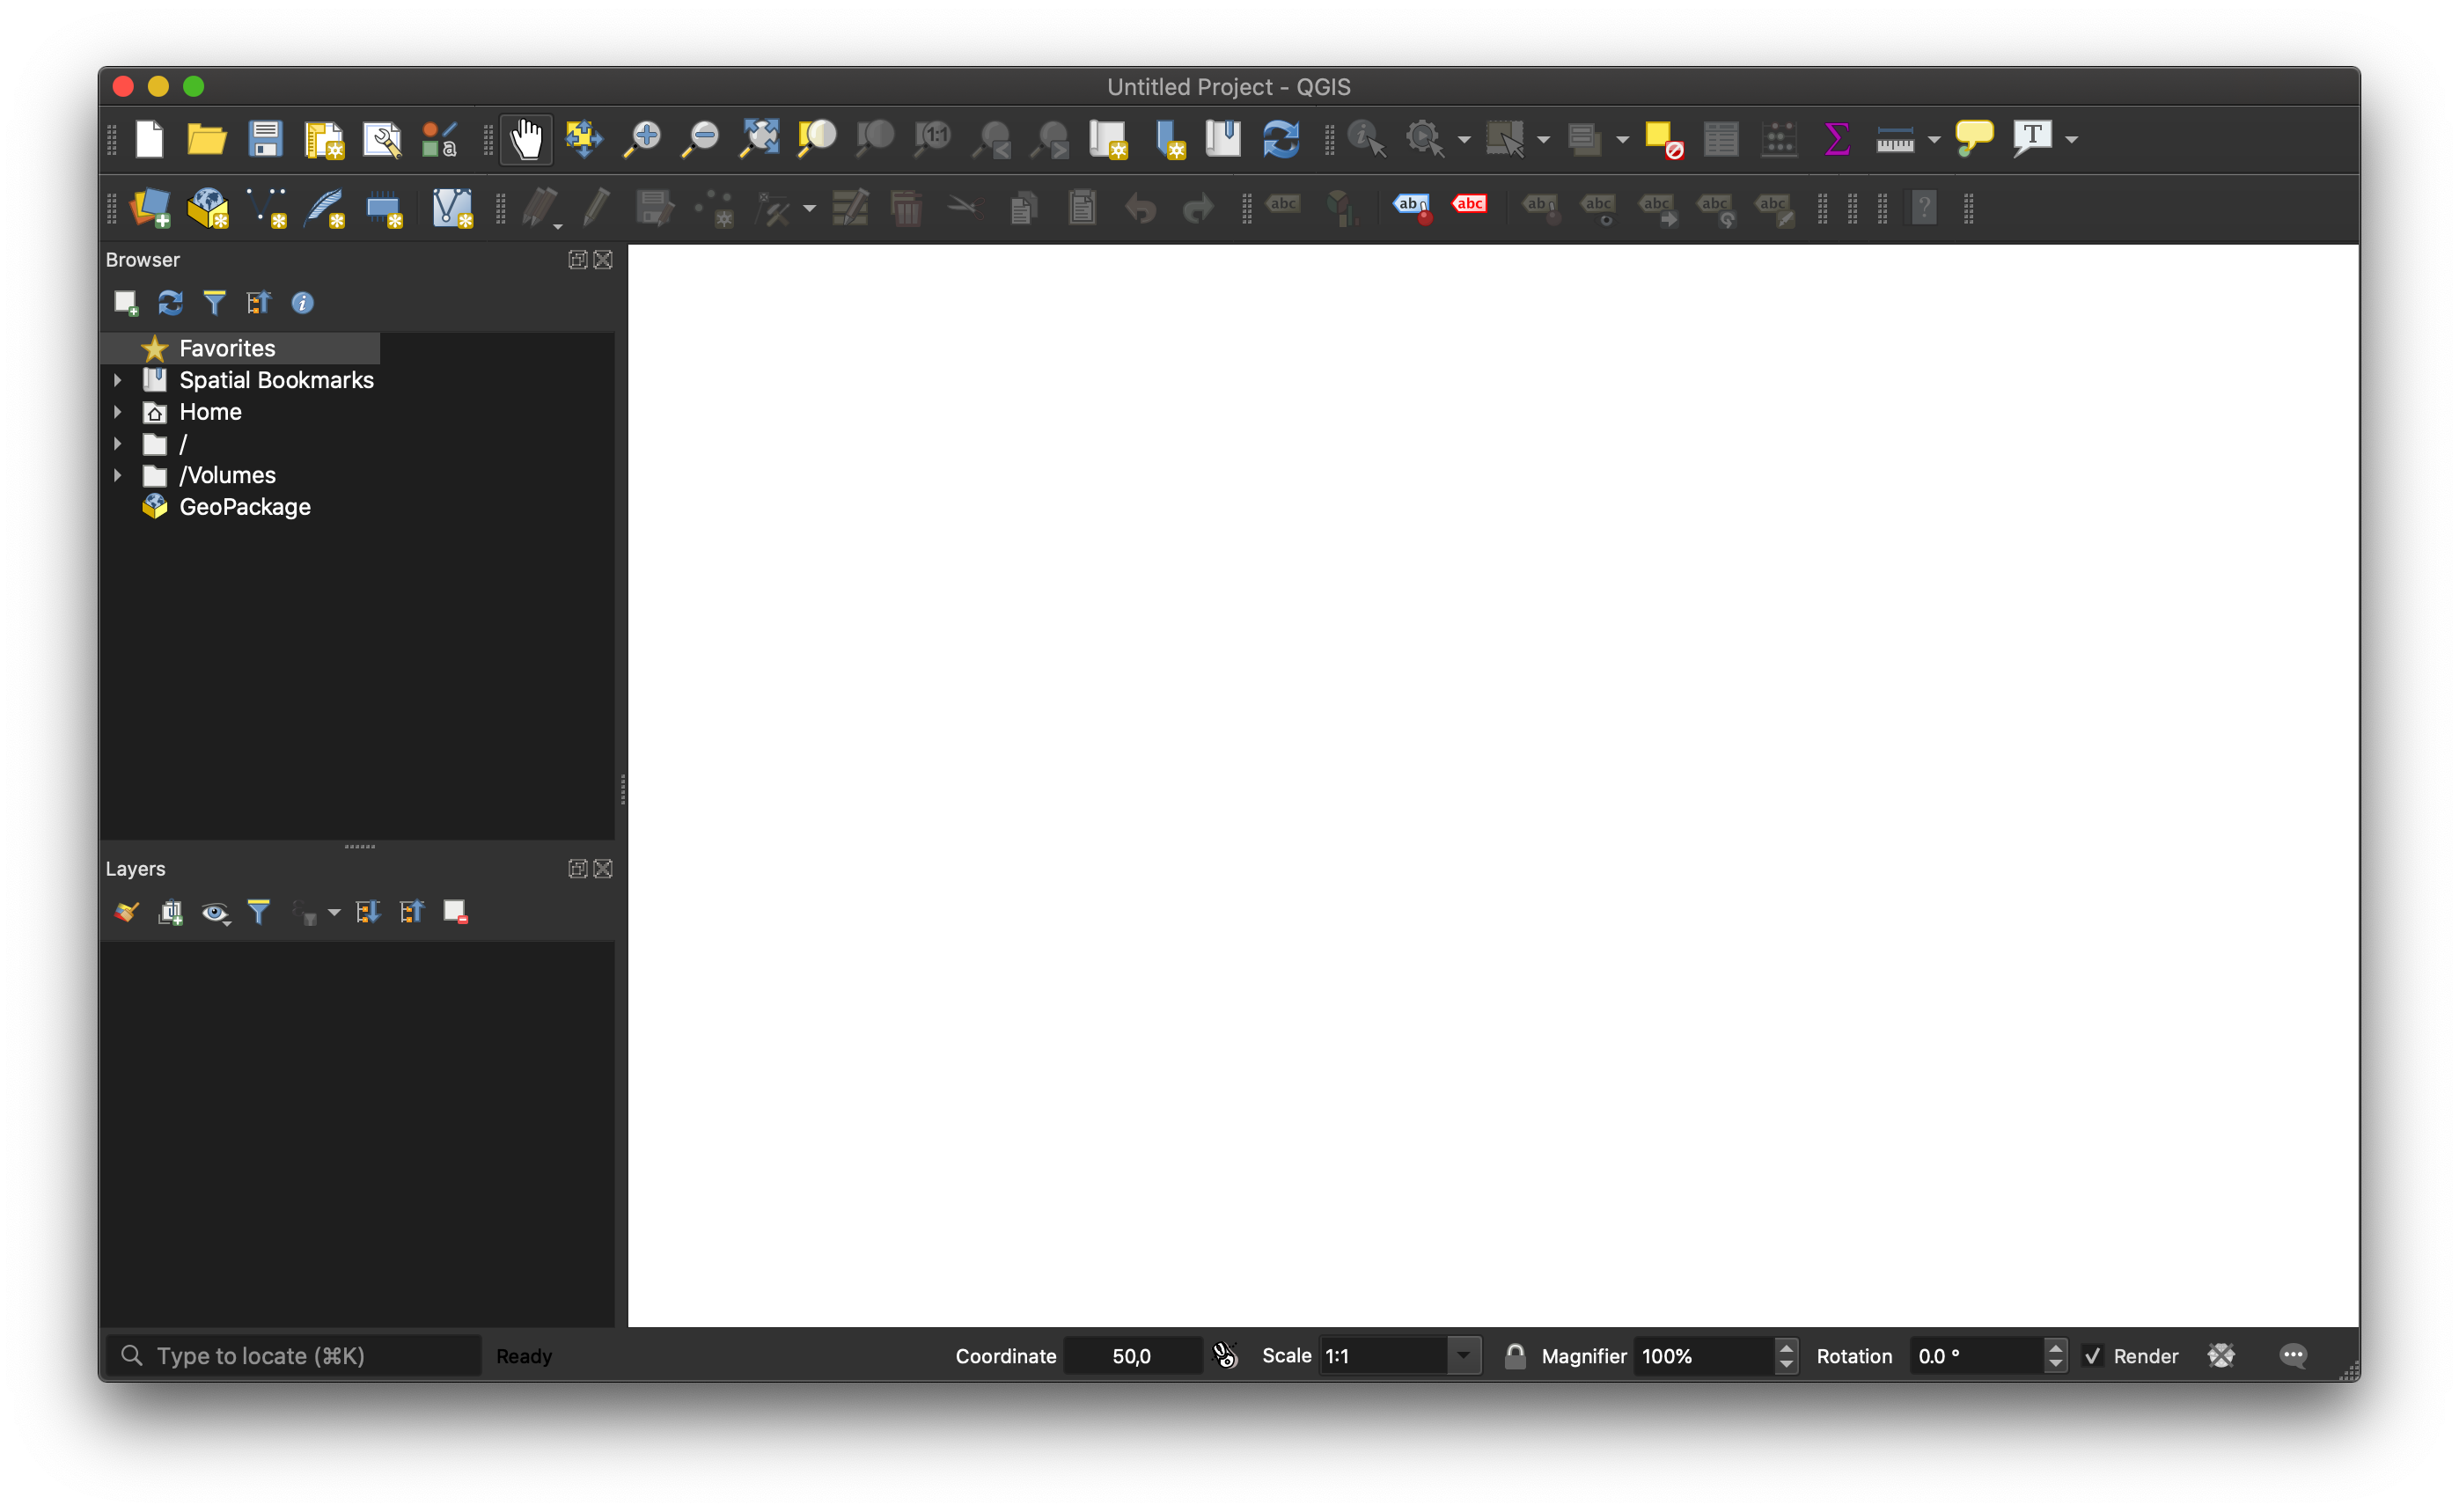
\includegraphics[scale=0.3]{images/analysis/qgis-project.png}
	\caption{Ansicht eines neuen leeren Projekts in QGIS}
	\label{fig:analysis-qgis-project}
\end{figure}
Man findet sich in einem komplett leeren Projekt ohne Kartenansicht und weißem Hintergrund.
Bei einigen Funktionen war nicht nachvollziehbar, was im Hintergrund passiert ist.
Beim Klick auf ``\emph{Project > New}`` oder ``\emph{Project > New from Template}`` ist nichts passiert und es war nicht klar, wie zu beginnen ist.
}{
Vom Hersteller selbst gibt es keine mobilen Anwendungen.
Auf der Downloadseite wird zwar auf eine veraltete Android-Anwendung verwiesen, die allerdings nicht für Touch-Interaktionen optimiert ist.
Außerdem wird darauf hingewiesen, dass die Anwendung Android Versionen ab der Version 5 nicht unterstützt, welche bereits 2014 veröffentlicht wurde \parencite{PIC2014}.
}{
Trotz möglicher kostenloser Benutzung handelt es sich bei QGIS um eine Anwendung mit einer langen Einarbeitungszeit.
Die Nutzung der Funktionen ist teilweise nicht nachvollziehbar und es werden keine mobilen Lösungen angeboten.
}

\subsection{Autodesk AutoCAD \& Civil}
Das Unternehmen Autodesk ist spezialisiert auf Software für 3D Planung und Konstruktion.
Mit den Programmen Autodesk AutoCAD und Autodesk Civil erhält man zwei mächtige CAD (Computer-aided design) und BIM (Building Information Modeling) Werkzeuge, um Indoor Maps zu erstellen.
\analysisresults{
Wie bereits in der Einleitung bei der Beschreibung der Problemstellung genannt betragen die Lizenzkosten für Autodesk AutoCAD 2.135 \text{€}/Jahr und für Autodesk Civil 2.315 \text{€}/Jahr (Stand: 14. Juli 2020, Autodesk).
Das von Autodesk genutzte Abomodell sorgt dafür, dass regelmäßig gezahlt werden muss, auch wenn die Software nicht genutzt wird.
Dieses Modell rentiert sich nicht für den Vermieter, da nach erster Fertigstellung der Kartendaten an dem Projekt nur selten Änderungen vorgenommen werden.
}{
Da es sich hierbei um eine auf Computer-aided design spezialisierte Software handelt, die vorwiegend im professionellen Bereich genutzt wird, ist auch mit einer langen Einarbeitungszeit zu rechnen.
\begin{figure}[h!]
	\centering
	\vspace{15pt}
	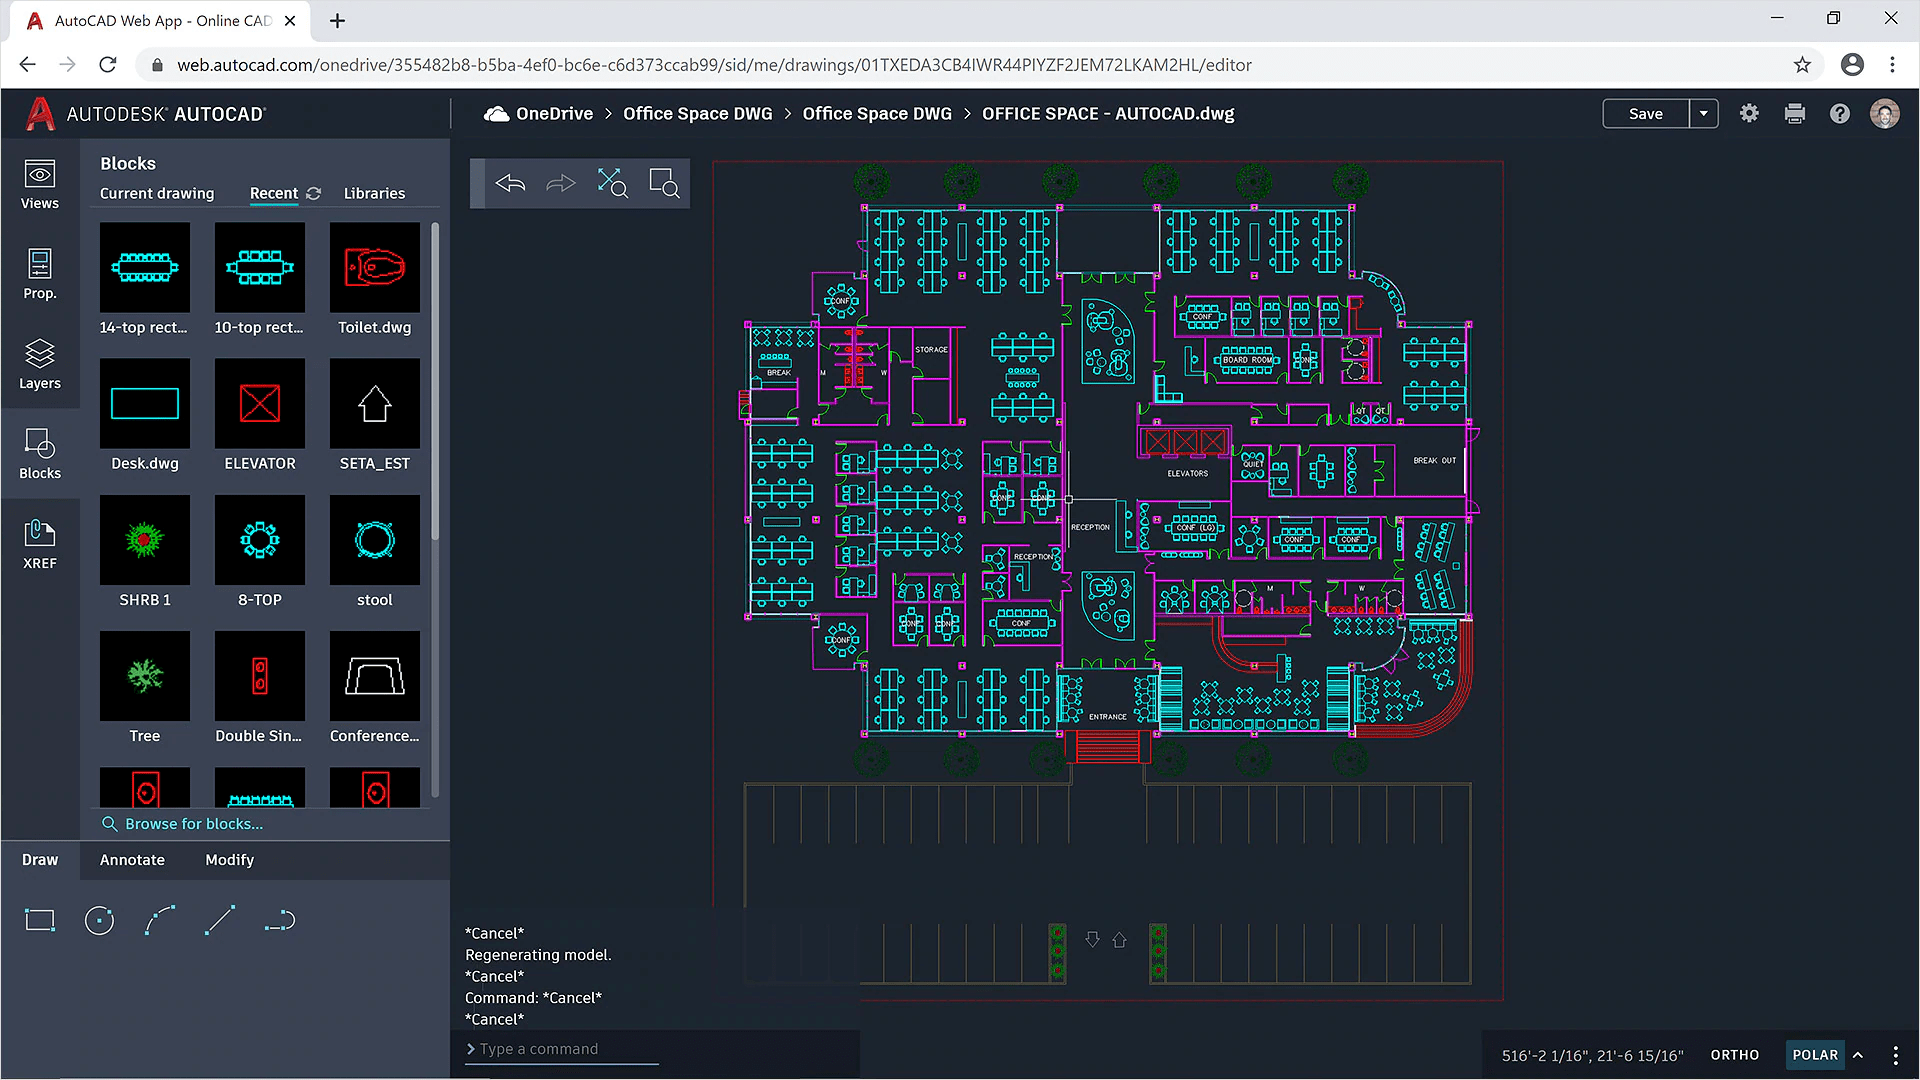
\includegraphics[scale=0.2]{images/analysis/autocad-web.png}
	\caption{Bearbeitungsansicht in der Autodesk AutoCAD Web App \parencite{AUT2020a}}
	\label{fig:analysis-autocad}
\end{figure}
Die vielen Details und Möglichkeiten, welche für eine CAD-Software von Nöten sind, sorgen für einen komplizierteren Einstieg.
Obwohl Autodesk ein \emph{Knowledge Network} mit Videos und Erklärungen zum Erlernen der Software bereitstellt, finden sich auf der Website eher Erklärungen zu speziellen Fällen anstatt zur grundlegenden Benutzung \parencite{AUT2020b}.
}{
Die Software Autodesk AutoCAD kann als Student oder Beschäftigter einer akademischen Einrichtung kostenlos getestet werden.
Da es bei der Verifizierung des Studentenstatus Probleme gab, konnte die Bedienung der Software nicht getestet werden.
}{
Autodesk bietet für AutoCAD zwar eine mobile Anwendung für iOS- und Android-Endgeräte an, allerdings werden diese auch mit einem Abomodell vertrieben.
Bei 60 \text{€} im Jahr \parencite{AUT2020} verstärkt dies auch hier die Problematik der preislichen Stemmbarkeit.
}{
Besonders aufgrund der hohen Kosten und der nötigen Einarbeitungszeit in das Computer-aided design ist Autodesk AutoCAD keine gute Lösung für den Vermieter.
Das Abomodell würde dafür sorgen, dass regelmäßig Kosten für den Vermieter anfallen, die seinerseits nicht gerechtfertigt sind.
}

\section{Dienstleistungslösungen}
Neben den Softwarelösungen zur Erstellung von Indoor Maps gibt es auch Dienstleistungslösungen.
Die Räumlichkeiten werden von den Dienstleistern vermessen und die Kartendaten ebenfalls von diesen erstellt.
Unter anderem bieten folgende Unternehmen Dienstleistungen für Indoor Navigation an:
\begin{itemize}
	\item https://www.infsoft.com/
	\item https://www.locuslabs.com/
	\item https://www.esri.com/en-us/arcgis/products/arcgis-indoors/overview
\end{itemize}
Einige weitere finden sich außerdem im Anhang der \emph{Community Standard Justification} des \acl{imdf}s \parencite{HOA2019}.
Bei der Kostenbestimmung der Dienstleistungslösungen können keine genauen Angaben getroffen werden, da die Kosten je nach Aufwand für den Dienstleister variieren.

\section{Probleme bei den vorhanden Lösungen}
Bei allen anlysierten Softwarelösungen handelte es sich nicht um eine Software zum Erstellen von Indoor Maps.
Mit Geographischen-Informationssystemen kann man im Allgemeinen mit Kartendaten arbeiten.
Darunter fällt zwar auch das Erstellen von Objekten, wie Punkte, Linien und Polygone, allerdings ohne jeglichen Bezug zu Indoor Maps.
Die Beziehungen zwischen den Objekten, wie sie im \acl{imdf} gewollt sind, können nicht sehr gut abgebildet werden.
Bei den CAD-Anwendungen besteht ein ähnliches Problem.
Dort wird zum Einen nicht direkt für Kartendaten gezeichnet, sondern eher die Grundrisse digital dargestellt, und zum Anderen besteht auch hier die Problematik, dass Beziehungen schlecht abgebildet werden können.\pbreak%
%
In beiden Fällen hat das zu bedeuten, dass die exportierten Informationen aus den Anwendungen noch einmal überarbeitet werden müssen.
Zwar finden sich auch \ac{imdf}-Export-Funktionen, allerdings können in diesem Export auch nur die Informationen abgebildet werden, die gezeichnet werden können.\pbreak%
%
Dienstleistungslösungen können diese Arbeit übernehmen.
Nachdem die Kartendaten in den entsprechenden Programmen erstellt wurden, kann der \ac{imdf}-Datensatz bearbeitet und angepasst werden.
Doch Dienstleistungslösungen sind vergleichsweise teuer und haben zusätzlich den Nachteil, dass bei Aktualisierungen der Kartendaten erneut Kosten entstehen, um den Dienstleister zu bezahlen.
